\documentclass{article}
\usepackage{amsmath,amsfonts,fancyhdr,parskip,amssymb,amsthm,graphicx}
\usepackage[margin = 1.5in]{geometry}
\usepackage[all]{xy}
\pagestyle{fancy}
\lhead{Ben Carriel (bkc39)}
\chead{Bryan Cuccioli (blc72)}
\rhead{Andy Levine (awl58)}
\setlength{\parindent}{1cm}

\DeclareMathOperator{\oh}{\mathcal{O}}
\DeclareMathOperator{\ta}{\xrightarrow{\ \ \ }}
\DeclareMathOperator{\opt}{\texttt{OPT}}

\newcommand{\problem}[1]{\noindent {\bf #1}}
\newcommand{\problempart}[1]{\noindent{\textbf{(#1)}}}

\newtheorem*{thm}{Theorem}
\newtheorem*{lem}{Lemma}
\newtheorem*{claim}{Claim}
\newtheorem*{defn}{Definition}
\newtheorem*{prop}{Proposition}

\begin{document}

\problem{Problem 1.} The counterexample is the following graph:

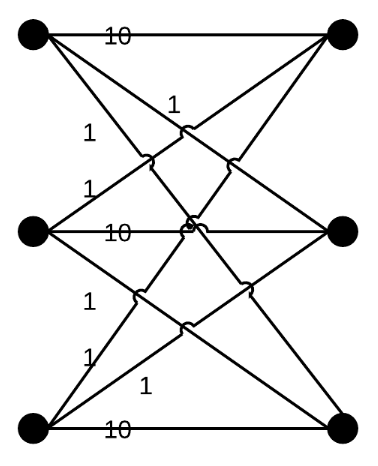
\includegraphics[width=50mm]{grapha.png}

\problem{Problem 2.} Observe first that the following graph is the ``worst case'' in the sense that the Hopcroft-Karp algorithm creates the least efficient matching for it. We will proceed via an induction-like argument. Define a `z-shaped subgraph' to be one that looks like the following:

\begin{displaymath}
\xygraph{
!{<0cm,0cm>;<1cm,0cm>:<0cm,1cm>::}
!{(0,0) }*+{\bullet_{a}}="a"
!{(1.5,0) }*+{\bullet_{b}}="b"
!{(0,1.5) }*+{\bullet_{c}}="c"
!{(1.5,1.5)}*+{\bullet_{d}}="d"
"a":"b"
"b":"c"
"c":"d"
}
\end{displaymath}

For $K_{2,2}$, then it is clear that the z-shaped subgraph is the worst case, because the other cases are just $K_{1,1}$ or two connected components made up of copies of $K_{1,1}$. Suppose now that for $K_{n-1,n-1}$, the worst case is a string of connected z-shaped subgraphs. Now considering $K_{n,n}$, adding two more vertices, we have the worst case matches them, because previously every node was matched with the one diagonally across from it. Hence the worst case matching is the one composed of a string of z-shaped subgraphs.

Then it is easy to see that $c_1=1/2$, because in the worst case the algorithm first chooses a path of length 1, and so in the worst case graph described above we have $|M_1|/|M^{\ast}|=1/2$.



On the second iteration, the algorithm picks blocking paths of size 2, and in the general $k$th step it picks blocking paths of size $k$. Hence the minimal matching is increasing by \emph{at least} 1 every iteration. We have $|M^{\ast}|$ as the least upper bound for $|M_k|$, so by a basic theorem of analysis, we must have $c_k\to 1$ as $k\to\infty$.

\problem{Problem 4.} 
\problempart{a} Fix a vertex $i \in L$ and let the event
\[
A_j = \{\text{vertex } i \text{ is matched with vertex } j \in R\}
\] 
Let's call a vertex matched if the edge $(i,j)$ is in the output of the stateless rounding procedure. Then 
\[
P(\{\text{vertex } i \text{ is matched}\}) = P( \bigcup_{j\in R} A_j )
\]
For a single event $A_k$ we have that 
\[
P(A_k) = x_{ik}z_k^{-1}
\]
But, because the events $A_k$ are not independent, we need to use the principle of inclusion-exclusion. This gives that
\[
P( \bigcup_{j\in R} A_j ) = \sum_{j \in R} (-1)^nP(\bigcap_{\substack{A \in S \\ |S| \leq |R| }}A)
\]
Where $S$ is some subset of $R$. In order to compute the terms on the right side of the equation we will use the following. 


\end{document}

